\chapter{Beispiele}
\section{Einbindung eines Bildes}
Ein Bild kann wie folgt eingebunden werden und wird automatisch ins Abbildungsverzeichnis aufgenommen:

\begin{figure}[htb]
  \centering
  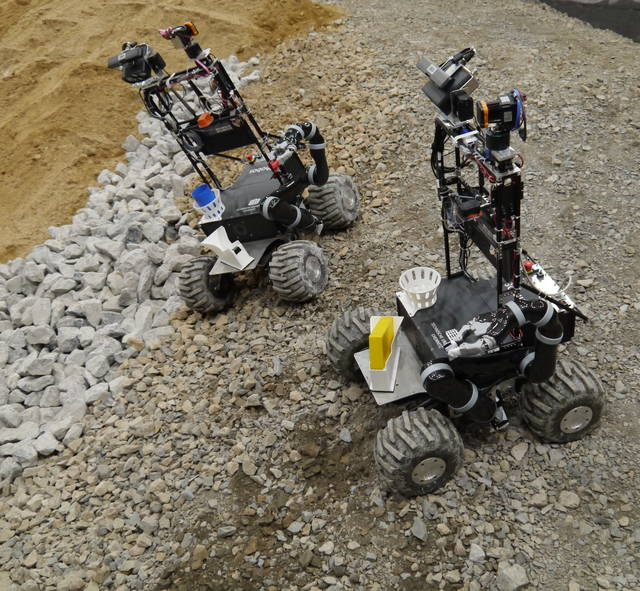
\includegraphics[width=0.75\textwidth]{beispiel.jpg}
  \caption{Die beiden Roboter Phobos und Deimos}
  \label{fig:roboter}
\end{figure}

Eine Referenz auf ein Bild wird wie folgt erzeugt: In Abbildung~\ref{fig:roboter} sind die beiden Roboter Phobos und Deimos dargestellt.

\section{Einbindung einer Tabelle}
Einbindung einer Tabelle:

\begin{table}[htb]
  \centering
  \begin{tabular}{l|c|r}
    Spalte 1 		& Spalte 2 	& Spalte 3 	\\
    linksbündig 	& zentriert 	& rechtsbündig 	\\
    1			& 2		& 3		\\
  \end{tabular}
  \caption{Eine Tabelle}
  \label{tab:table1}
\end{table}

Die Tabelle~\ref{tab:table1} ist nur ein minimales Beispiel.

\section{Angabe einer Literatur-Quelle}
Mehr Informationen über die Roboter der Professur Prozessautomatisierung können beispielsweise in \autocite{robots} gefunden werden. Dazu müssen die Informationen zur Quelle im Bibtex-Style in die Datei \textit{literatur.bib} eingefügt werden.



